\documentclass[conference]{IEEEtran}
\IEEEoverridecommandlockouts
\usepackage{amsmath,amssymb}
\usepackage{graphicx}
\usepackage{cite}
\usepackage{booktabs}
\usepackage{textcomp}

\renewcommand{\dbltopfraction}{0.95}
\renewcommand{\dblfloatpagefraction}{0.85}

\begin{document}

\title{PRISM: One-Sided CSI Feedback for 5G NR via a Published Mixture of Karhunen--Lo\`{e}ve Sketches}

\author{
\IEEEauthorblockN{Author Name\IEEEauthorrefmark{1}}
\IEEEauthorblockA{\IEEEauthorrefmark{1}Department of Electrical and Computer Engineering, University Name, City, Country\\
Email: author@university.edu}
}

\maketitle

\begin{abstract}
The 3GPP Type II codebooks spend many feedback bits because they describe the channel on a fixed DFT grid. Learned CSI feedback can do better, but the usual two-sided autoencoders put a neural network on the UE and force UE and gNB vendors to train and version-match a shared model. We present PRISM, a one-sided scheme with zero learned parameters on the UE and no neural network anywhere. The idea is simple: a cell serves line-of-sight and non-line-of-sight users at the same time, so we publish a small dictionary of $K$ Karhunen--Lo\`{e}ve (KLT) bases, one per propagation regime, fitted offline by subspace clustering. Per report, the UE projects the eigen-precoder onto each basis, keeps the one that captures the most energy, and signals its index with two bits ($K{=}4$). The gNB reconstructs with one matrix multiply (least squares). On a mixed Sionna 38.901 bank that draws equally from CDL-A through E, PRISM needs 50--57\% fewer bits than the best codebook at the same accuracy, reaches SGCS 0.977 at 146 bits where the best codebook stops at 0.937, and also wins on every single profile. A variant fitted without CDL-E still scores 0.972 on it.
\end{abstract}

\begin{IEEEkeywords}
CSI feedback, massive MIMO, Karhunen--Lo\`{e}ve transform, mixture models, subspace clustering, 5G NR
\end{IEEEkeywords}

\section{Introduction}
In FDD massive MIMO, the gNB needs channel state information (CSI) that only the UE can measure, so the UE must feed it back over a costly uplink control channel. The 3GPP Type II codebooks~\cite{3gpp38214} encode the precoder as a set of DFT beams and delay taps with quantized weights. This works, but it is expensive: on our mixed-profile deployment benchmark the codebooks need more than 100 bits per report to pass 0.90 mean SGCS, and every report re-sends the beam and tap choices from scratch.

Machine-learned CSI feedback promises much better compression. The best-known family, the CsiNet-style autoencoders~\cite{wen2018csinet,guo2022overview}, learns an encoder for the UE and a decoder for the gNB together. This design has two well-known deployment problems. First, the UE must run a neural network, which costs power and chip area. Second, the encoder and decoder are one model split across two vendors, so the vendors must train together and keep their halves in sync -- a coordination problem 3GPP has not solved. A third problem gets less attention but is just as real: a learned scheme is fitted to a channel distribution, and a real cell does not have one distribution. It serves line-of-sight (LoS) and rich-scattering users side by side. A model fitted to one group loses accuracy on the other.

PRISM (Precoder Reporting via an Indexed Sketch Mixture) is built to avoid all three problems at once:
\begin{itemize}
\item \textbf{No neural network anywhere.} The UE encoder is a few fixed matrix multiplies; the gNB decoder is one fixed matrix multiply. The only ``learned'' objects are $K$ constant matrices, estimated offline from channel statistics and published like a codebook table.
\item \textbf{One-sided by construction.} Nothing trained crosses the air interface or the vendor boundary. UE and gNB only need to agree on the published constants, which is less than agreeing on a codebook.
\item \textbf{Built for mixed channel populations.} PRISM publishes a small \emph{mixture} of $K$ Karhunen--Lo\`{e}ve (KLT) bases, one per propagation regime, and the UE picks the best basis for each report at the price of $\lceil\log_2 K\rceil$ bits. The fitting step finds the regimes by itself, with no labels.
\end{itemize}
The mixture is the key point. A single KLT basis is the best linear sketch for \emph{one} channel distribution~\cite{eckartyoung1936}. When the data is a mix of regimes, a single basis fitted on everything is optimal for none of them -- we measure this ``averaging penalty'' directly in Sec.~\ref{sec:results}. One basis per regime, plus a cheap per-report choice, removes the penalty. This idea has classical roots: universal transform coding selects among several KLTs per block~\cite{effros1995wutc}, and fitting the bases is a subspace-clustering problem~\cite{tipping1999mppca,vidal2011subspace}. PRISM packages these tools for the one-sided CSI constraint. Because everything published is a table of constants, PRISM is, in spirit, exactly what 3GPP already standardizes: a codebook -- here, a codebook of transforms.

We evaluate against all 28 configurations of the R15--R17 codebook family (Type I, Type II, eType II, FeType II) on identical frozen Sionna~\cite{sionna} 38.901~\cite{3gpp38901} channel banks -- most importantly a \emph{mixed} bank that draws equally from CDL-A through CDL-E, the deployment-level test a single-profile evaluation hides.

\section{System Model and the Codebook Baseline}
Let $H[t,r,p]$ be the downlink channel for subband $t\in\{1,\dots,N_3\}$, receive antenna $r$, and transmit port $p\in\{1,\dots,P\}$ of an $(N_1,N_2)$ dual-polarized array. For rank $v$, the UE computes the dominant right singular vector of $H[t]$ per subband (it already does this for CQI reporting) and aligns the arbitrary per-subband phases sequentially across $t$. The result is the eigen-precoder $V\in\mathbb{C}^{N_3\times P\times v}$ with unit-norm columns. Every PMI scheme, codebook or learned, is an approximation of $V$; we score all of them with the squared generalized cosine similarity (SGCS) between $V$ and the reconstruction, and with the downlink spectral efficiency (SE) it produces.

The Type II codebooks approximate $V$ as a weighted sum of $L$ selected DFT beams and $M_v$ selected delay taps. Each report carries the beam indices, the tap window, a bitmap of non-zero weights, and the quantized weights. Three costs follow. The support (which beams, which taps) is re-encoded in every report. Real propagation paths rarely sit exactly on the DFT grid, so their energy leaks over many beams and taps, which forces larger $L$ and $M_v$. And the weight quantizer spends the same number of bits on every coefficient. PRISM avoids all three costs by measuring the channel's own principal directions instead of assuming a grid.

\section{The PRISM Method}
\subsection{The Sketch Report}
PRISM first moves $V$ into the angle--delay domain: a unitary 2-D spatial DFT over the $(N_1,N_2)$ port grid and a unitary IDFT along frequency~\cite{wen2018csinet}, flattened to a vector $g\in\mathbb{C}^{D}$, $D=PN_3$. In this domain each physical path concentrates into few coordinates.

The report is a \emph{sketch}: $y = A[{:}m]\,g$, the projection of $g$ onto the top $m$ rows of a fixed basis $A$. We use the KLT basis -- the eigenvectors of the second-moment matrix $\mathbb{E}[gg^H]$, ordered by variance -- because it is the linear map that keeps the most energy of any $m$-row sketch~\cite{eckartyoung1936}. Each coordinate is divided by its published standard deviation $\sigma_k$ (the square root of the KLT eigenvalue) and digitized with a fixed Lloyd--Max quantizer of the standard normal~\cite{lloyd1982,max1960}. A total budget of $2mB$ bits is spread over the $2m$ real dimensions by reverse water-filling~\cite{coverthomas2006,gershogray1992}: high-variance coordinates get more bits, negligible ones get none. The allocation is a fixed function of the published $\sigma$, so the gNB computes the same allocation and no side information is sent. Because the rows of $A$ are ordered by variance, any prefix of a report is a valid smaller report: the payload can be cut to fit any uplink grant, and the same decoder still works (a \emph{rateless} report). All of this is fixed at design time; the UE trains nothing.

\subsection{Why One Basis Is Not Enough, and the Mixture}
A KLT basis is matched to one distribution. A cell's channel population is a mixture: near-LoS channels are dominated by one specular path; rich-scattering channels spread energy over many paths. Their second-moment matrices differ, so no single basis serves both well. Fitting one basis on pooled data does not help much -- it pays an averaging penalty on every regime (measured in Sec.~\ref{sec:results}).

PRISM therefore publishes $K$ basis--scale pairs $\{(A_k,\sigma_k)\}_{k=1}^{K}$. For each report the UE computes
\begin{equation}
k^{*} = \arg\max_{k} \bigl\lVert A_k[{:}m]\, g \bigr\rVert^2 ,
\label{eq:select}
\end{equation}
the basis that captures the most energy of $g$ in its $m$-row sketch. Since the rows of each $A_k$ are orthonormal, the captured energy is exactly what a least-squares decoder recovers, so \eqref{eq:select} directly picks the basis that reconstructs best. The report is $\lceil\log_2 K\rceil$ index bits plus the $2mB$-bit sketch quantized under basis $k^*$'s published allocation. The UE-side cost is $K$ matrix multiplies and an argmax -- the winner's sketch is already computed during the selection. A cheaper two-stage rule selects on a short $m_{\mathrm{sel}}$-row prefix first and computes only the winner's full sketch.

The gNB reconstructs with one matrix multiply,
\begin{equation}
\hat g = A_{k^*}[{:}m]^{H}\, y ,
\label{eq:ls}
\end{equation}
the exact minimum-norm least-squares inverse (the rows are orthonormal), then maps $\hat g$ back through the inverse angle--delay transform and normalizes to the standard precoder convention $\mathrm{tr}(W^HW)=1$. PRISM is fully linear end to end. A gNB vendor may still add any decoder it likes (the report does not change), but none is needed.

\subsection{Fitting the Mixture Offline}
The $K$ bases are fitted once, offline, on eigen-precoder vectors $\{g_i\}$ collected from a training mix that covers the deployment's regimes. We alternate two steps until the assignment stops changing (K-subspaces clustering, Lloyd's algorithm applied to subspaces~\cite{tipping1999mppca,vidal2011subspace}):
\begin{equation}
\begin{aligned}
\text{assign: } & c_i \leftarrow \arg\max_k \lVert A_k[{:}m_{\mathrm{ref}}]\, g_i \rVert^2,\\
\text{refit: } & A_k \leftarrow \mathrm{KLT}\bigl(\{g_i : c_i = k\}\bigr),
\end{aligned}
\label{eq:ksub}
\end{equation}
with $m_{\mathrm{ref}}{=}16$, the same prefix length the UE uses for two-stage selection. The mean captured energy cannot decrease in either step, so the loop converges; we keep the best of several restarts. Initialization matters: starting from a random assignment fails, because every random half of the data has the same pooled covariance, so all $K$ components start identical and \eqref{eq:ksub} never separates them. We instead seed the first basis from a small random subset and each next basis from the samples the current set of bases captures \emph{worst} -- the k-means++ idea carried over to subspaces. The resulting split is reproducible -- five independent seeds converge to the same clusters and the same objective -- but is sensitive to $m_{\mathrm{ref}}$ itself: the clean LoS/NLoS separation reported below holds at $m_{\mathrm{ref}}{=}16$ and degrades toward mixed clusters at both $m_{\mathrm{ref}}{=}8$ and $m_{\mathrm{ref}}{=}32$, so $m_{\mathrm{ref}}$ should be treated as a fitted hyperparameter, not a free choice.

Fitted on 72{,}000 training vectors (48k from CDL-A/B/C, 24k from CDL-D/E), the $K{=}4$ mixture finds the physics on its own at this $m_{\mathrm{ref}}$: one cluster is 99\% CDL-D, one is 95\% CDL-E, and the remaining two split the rich-scattering profiles. No labels were given. Captured energy at $m{=}16$ reaches 94.5\% (A/B/C), 98.6\% (D), and 98.2\% (E), against 90.9\%, 94.6\%, and 85.4\% for a single pooled basis. Two components are not enough -- at $K{=}2$ both clusters stay mixtures and the LoS/NLoS split does not appear; it appears at $K{=}4$, and $K{=}8$ adds almost nothing (Sec.~\ref{sec:results}). We use $K{=}4$: two index bits.

\section{Complexity}
Table~\ref{tab:complexity} counts complex multiply--accumulates for the UE encoder at $K{=}4$, $m{=}16$, next to the R16 eType II beam search it replaces ($L{=}4$, $M_v{=}2$, oversampling $O_1{=}O_2{=}4$). The per-subband eigenvector step is excluded from both, since every PMI scheme needs it for CQI anyway. PRISM costs $KmD$ MACs and scales as $O(P)$; the codebook search scans oversampled beam groups and scales as $O(P^2)$, so PRISM's advantage grows with the array. The UE stores $K$ constant matrices and one quantizer table -- static ROM, the same kind a codebook needs -- and zero learned parameters. The gNB runs one matrix multiply.

\begin{table}[t]
\centering
\caption{UE encode cost, complex MACs ($K{=}4$, $m{=}16$)}
\label{tab:complexity}
\begin{tabular}{@{}lrrrrr@{}}
\toprule
Array & $P$ & PRISM & two-stage & R16 \texttt{select} & speedup \\
\midrule
(4,2)  & 16  & 8{,}228  & 4{,}132  & 17{,}440    & 2.1$\times$ / 4.2$\times$ \\
(4,4)  & 32  & 16{,}420 & 8{,}228  & 67{,}104    & 4.1$\times$ / 8.2$\times$ \\
(16,2) & 64  & 32{,}804 & 16{,}420 & 264{,}736   & 8.1$\times$ / 16.1$\times$ \\
(16,4) & 128 & 65{,}572 & 32{,}804 & 1{,}053{,}216 & 16.1$\times$ / 32.1$\times$ \\
\bottomrule
\end{tabular}
\end{table}

\section{Simulation Setup}
We use Sionna's~\cite{sionna} implementation of the 3GPP TR 38.901 CDL channels~\cite{3gpp38901}: a $(4,4)$ dual-polarized array ($P{=}32$), $N_3{=}8$ subbands, 2 receive antennas, rank 1. The mixture is fitted on 72{,}000 training vectors drawn from CDL-A through E with delay spread randomized over 30--300\,ns and UE speed over 3--30\,km/h per drop, as described above. Evaluation uses a single fixed operating point, 100\,ns delay spread and 3\,km/h, so the reported gains are not inflated by matching a wide training range at test time; delay spread and UE speed do not otherwise vary the rank-1, single-slot metric we score.

Every scheme -- all 28 configurations of the R15--R17 codebook family and every PRISM variant -- is scored on the \emph{same} frozen banks of channel drops through one evaluation harness, with bit-exact overhead accounting (the packed bitstream length must equal the claimed overhead). The main bank is \textbf{mixed}: 40 drops from each of CDL-A/B/C/D/E, interleaved deterministically, 200 drops total. This models a cell that serves all user types at once. We also report each profile alone (200 drops on CDL-C, 150 elsewhere) to show there is no weak spot hiding inside the average.

\section{Results and Ablations}
\label{sec:results}

\begin{figure*}[t]
\centering
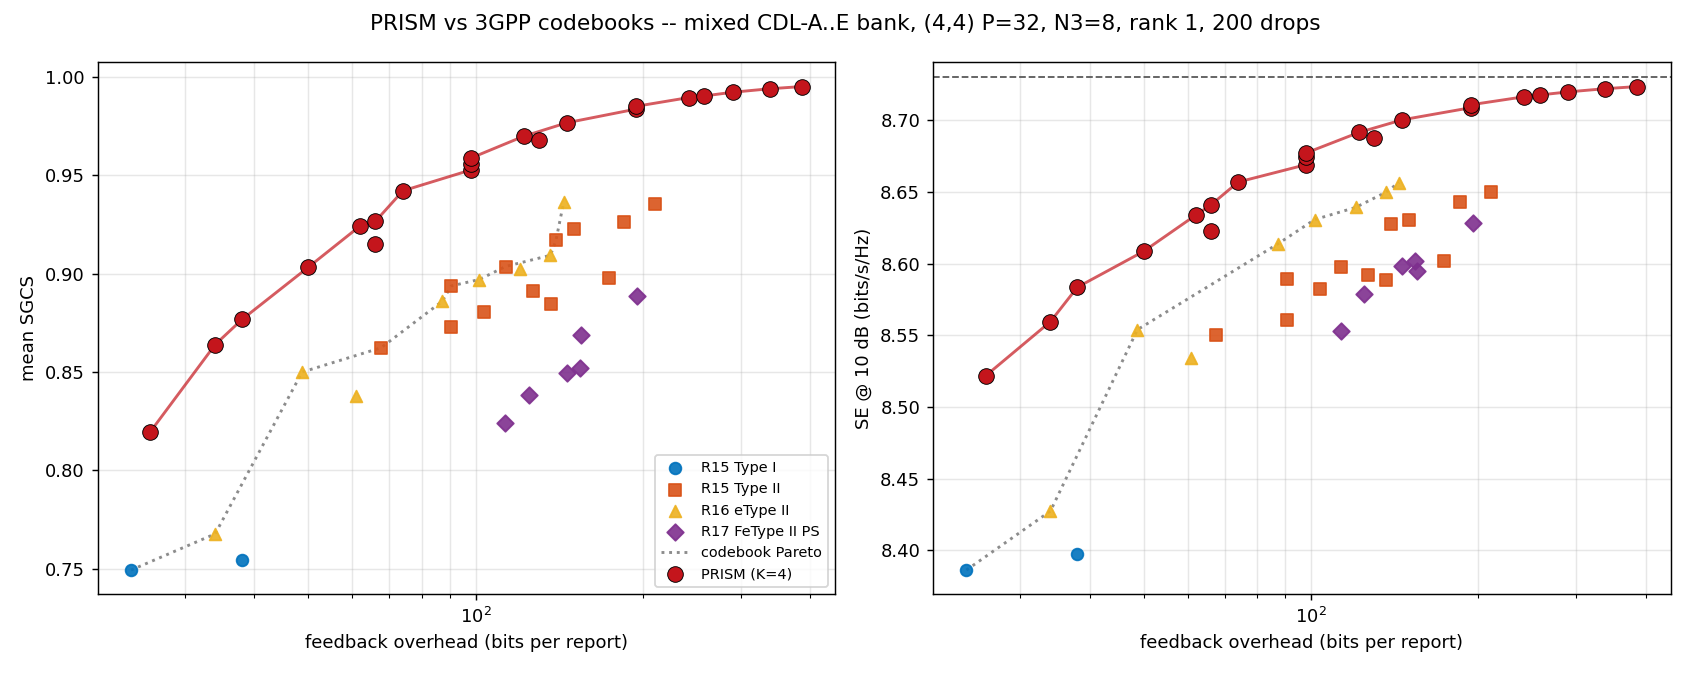
\includegraphics[width=0.98\textwidth]{figs/fig_paper_frontier.png}
\caption{Rate--distortion on the mixed CDL-A..E bank (200 drops): mean SGCS (left) and SE at 10\,dB (right) vs.\ feedback bits. Every codebook configuration is shown; the dotted line is the codebook Pareto frontier. PRISM sits above it over the whole range.}
\label{fig:frontier}
\end{figure*}

\textbf{Mixed-bank frontier.} Figure~\ref{fig:frontier} is the deployment-level comparison. PRISM's operating curve lies above the codebook Pareto frontier at every overhead. The best codebook result on the mixed bank is SGCS 0.937$\pm$0.003 (R16 eType II, 144 bits, $\pm$ one standard error of the mean over 200 drops throughout); PRISM reaches parity with it by 74 bits (0.942$\pm$0.004, within one standard error) and clearly exceeds it by 146 bits (0.977$\pm$0.002, a 12-standard-error gap) and 0.995 at 386 bits. At 194 bits PRISM's spectral efficiency is within 0.021 bits/s/Hz of the ideal-CSI upper bound (a 0.5\% relative gap; the matched-bits SE advantage over the best codebook at 144--146 bits is likewise under 1\% in this single-user, rank-1 setting, well below the SGCS gap in relative terms -- we expect the SGCS gap to matter more directly in an interference-limited MU-MIMO regime, which we do not evaluate here). At the small end, a 26-bit PRISM report scores 0.820 against 0.749 for the 24-bit Type I report, and PRISM can place a report at any bit count in between -- the codebooks only offer a fixed menu of sizes.

\begin{table}[t]
\centering
\caption{Bits to reach a target mean SGCS, mixed bank (``--'': unreachable)}
\label{tab:gain_mixed}
\begin{tabular}{@{}lccc@{}}
\toprule
Target SGCS & Best codebook & PRISM & Saving \\
\midrule
0.85 & 68  & 34  & $-$50\% \\
0.90 & 113 & 50  & $-$56\% \\
0.92 & 144 & 62  & $-$57\% \\
0.95 & --  & 98  & \\
0.97 & --  & 146 & \\
\bottomrule
\end{tabular}
\end{table}

\textbf{Overhead at matched accuracy.} Table~\ref{tab:gain_mixed} reads the same data the other way: to reach a given accuracy on the mixed bank, PRISM needs 50--57\% fewer feedback bits than the cheapest codebook that gets there, and above SGCS 0.94 no codebook configuration gets there at all. The 0.85 row is the closest call: the runner-up codebook configuration (R16 eType II, 49 bits) misses the 0.85 threshold by 0.00003, three orders of magnitude inside its own standard error ($\pm$0.006), so a different random seed could plausibly move that row's ``68'' to ``49'' -- we report the threshold as computed rather than adjust for this, and flag it so the reader can weigh it accordingly. Every other row in Tables~\ref{tab:gain_mixed}--\ref{tab:profiles} clears its comparison by several standard errors.

\begin{figure}[t]
\centering
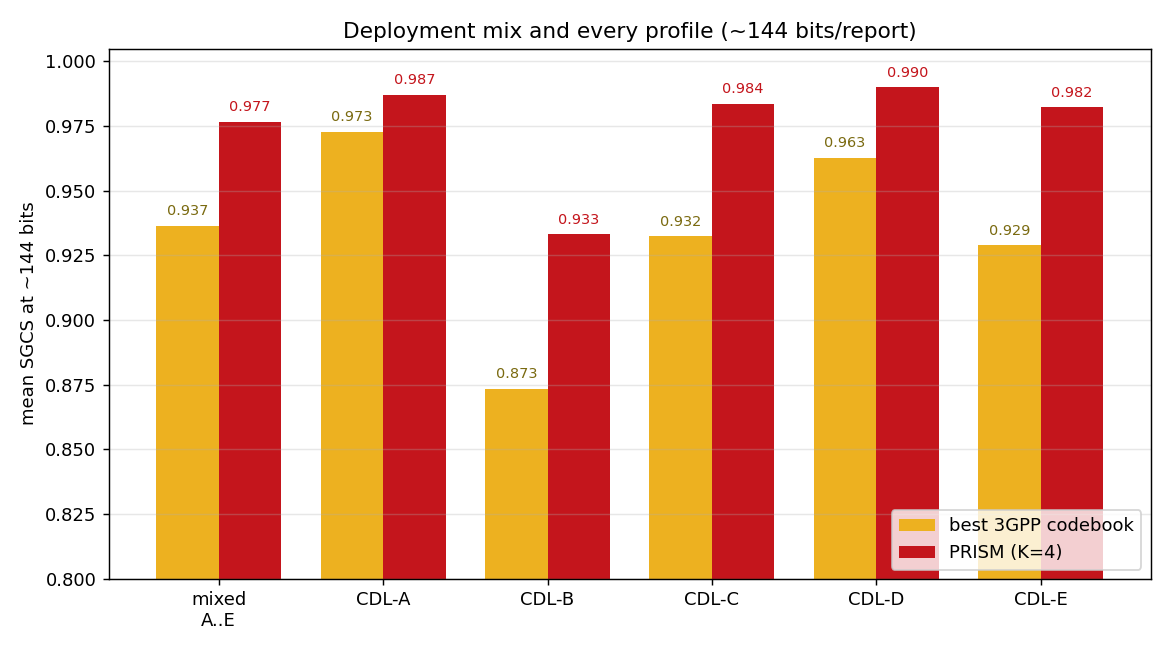
\includegraphics[width=0.98\linewidth]{figs/fig_paper_profiles.png}
\caption{Mean SGCS at $\approx$144 bits: the mixed bank and each CDL profile alone. PRISM wins in the mix and on every profile.}
\label{fig:profiles}
\end{figure}

\begin{table}[t]
\centering
\caption{Mean SGCS at $\approx$144 bits per report}
\label{tab:profiles}
\begin{tabular}{@{}lccc@{}}
\toprule
Bank & Best codebook & PRISM ($K{=}4$) & Gap \\
\midrule
mixed A..E & 0.937 & \textbf{0.977} & $+$0.040 \\
CDL-A & 0.973 & \textbf{0.987} & $+$0.014 \\
CDL-B & 0.873 & \textbf{0.933} & $+$0.060 \\
CDL-C & 0.932 & \textbf{0.984} & $+$0.052 \\
CDL-D & 0.963 & \textbf{0.990} & $+$0.027 \\
CDL-E & 0.929 & \textbf{0.982} & $+$0.053 \\
\bottomrule
\end{tabular}
\end{table}

\textbf{Every profile, not just the average.} A mixed-bank win could hide a weak profile inside the average. Figure~\ref{fig:profiles} and Table~\ref{tab:profiles} show it does not: at $\approx$144 bits PRISM beats the best codebook on all five profiles, by $+$0.014 (CDL-A, where codebooks are already strong) up to $+$0.060 (CDL-B). The worst profile under PRISM (0.933) is still better than the \emph{average} codebook behavior on the mix. Per profile, the savings at matched accuracy follow the same pattern as the mixed bank: on CDL-C, 62 bits vs.\ 161 for SGCS 0.92 ($-$61\%); on CDL-D, 34 vs.\ 65 ($-$48\%); on CDL-E, 62 vs.\ 117 ($-$47\%).

\begin{figure*}[t]
\centering
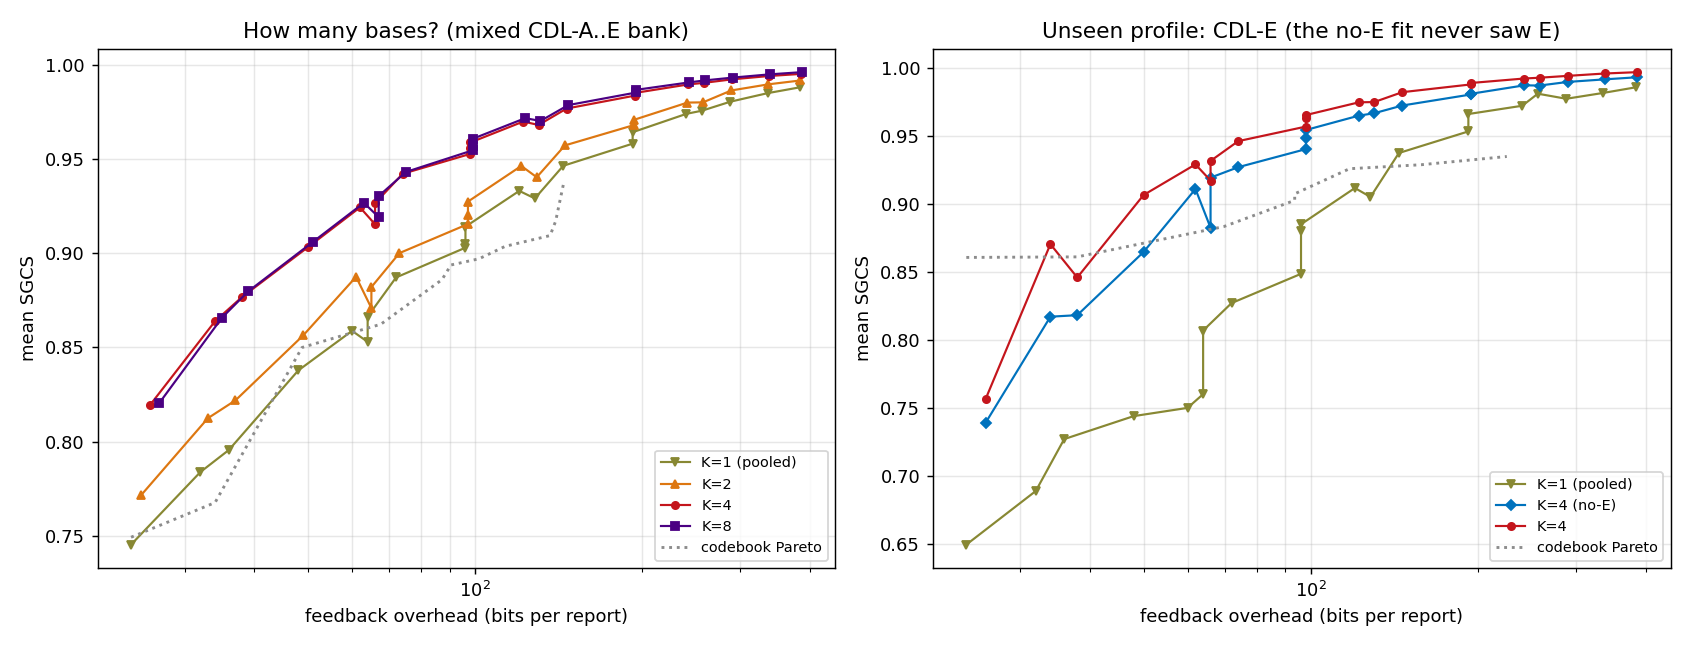
\includegraphics[width=0.98\textwidth]{figs/fig_paper_ablation.png}
\caption{Ablations. Left: number of bases on the mixed bank -- one pooled basis ($K{=}1$) only tracks the codebook frontier; the jump comes at $K{=}4$; $K{=}8$ adds nothing. Right: CDL-E when the fit never saw CDL-E -- the no-E mixture still beats the codebook frontier.}
\label{fig:ablation}
\end{figure*}

\textbf{Why the mixture matters (ablation).} Figure~\ref{fig:ablation} (left) varies $K$ on the mixed bank. At $\approx$98 bits: $K{=}1$ scores 0.903, $K{=}2$ 0.915, $K{=}4$ 0.953, $K{=}8$ 0.955. Two things stand out. First, the single pooled basis ($K{=}1$) -- the same data, the same quantizer, just no mixture -- only roughly \emph{tracks} the codebook frontier. Nearly the entire gap between PRISM and the codebooks comes from the mixture, not from the KLT alone. Second, $K{=}2$ recovers little, because its two clusters fail to separate the LoS and NLoS regimes; the clean split appears at $K{=}4$ and saturates there. The 2 index bits of $K{=}4$ buy $+$0.05 SGCS at fixed overhead.

\section{Generalization and Limits}
\textbf{Unseen profile.} We refit the mixture with every CDL-E sample removed and evaluated it on CDL-E (Fig.~\ref{fig:ablation}, right). The no-E mixture scores 0.972 at $\approx$144 bits -- above the best codebook (0.929) and within 0.010 of the full mixture (0.982). The cluster fitted on CDL-D covers CDL-E, because both are near-LoS: what must be covered is the propagation \emph{regime}, not the exact profile. This weakens the usual objection to learned CSI (``you cannot anticipate every channel'') to a much easier requirement: cover every regime.

\textbf{Measured limits.} Four limits are visible in our data and worth stating plainly. First, at low accuracy targets on near-LoS channels, the 24-bit Type I report is hard to beat: a specular channel \emph{is} one DFT beam, and a one-beam index is the perfect code for it (on CDL-E, Type I reaches SGCS 0.85 with 24 bits; PRISM needs 34). This niche is small but real. Second, a propagation regime absent from the fit entirely -- neither rich-scattering nor near-LoS -- would degrade PRISM toward its pooled-basis floor. The failure is graceful (Fig.~\ref{fig:ablation} left shows that floor still tracks the codebooks), and a codebook fallback always exists. Third, the published dictionary is tied to one antenna geometry $(N_1,N_2,N_3)$; a network fits one dictionary per array type. This is a gNB-side artifact -- the UE just stores the constants it is told to -- but it does multiply the standardization surface by the number of geometries. PRISM also reports the current eigen-precoder only; CSI aging and channel prediction are separate problems. Fourth, the $\lceil\log_2 K\rceil$-bit basis index is reported without redundancy: at $K{=}4$ every 2-bit pattern names a valid basis, so an undetected uplink bit error on the index silently selects the wrong published basis -- wrong scale, wrong bit allocation, wrong inverse transform -- rather than degrading gracefully. A deployment would need to protect this header the way RI/CQI already are (e.g.\ a short CRC or a channel code), which we have not evaluated here.

\section{Conclusion}
PRISM shows that the gains of learned CSI feedback do not require a neural network, a learned UE encoder, or joint vendor training. One published object -- a small dictionary of KLT sketch bases, fitted offline by subspace clustering on a regime-covering mix -- with a two-bit per-report basis choice is enough to beat every configuration of the 3GPP R15--R17 codebook family on a realistic mixed channel population (50--57\% fewer bits at matched accuracy) and on every individual CDL profile at the same time. The fit discovers the LoS/NLoS structure without labels; the report is rateless; the UE encoder is cheaper than the codebook search it replaces; and the gNB decoder is one matrix multiply. The measured limits -- a small Type I niche at low rate on specular channels, and regimes absent from the fit -- come with graceful fallbacks. The general lesson: when a learned component must be standardized across vendors, publish a small mixture of linear maps and let a few signalled bits pick among them. It keeps most of the learning gain and none of the deployment cost.

\bibliographystyle{IEEEtran}
\begin{thebibliography}{15}

\bibitem{3gpp38214}
3GPP, ``NR; Physical layer procedures for data,'' 3GPP TS 38.214, V19.4.0, Release 19.

\bibitem{3gpp38901}
3GPP, ``Study on channel model for frequencies from 0.5 to 100 GHz,'' 3GPP TR 38.901.

\bibitem{sionna}
J. Hoydis \emph{et al.}, ``Sionna: An open-source library for next-generation physical layer research,'' arXiv:2203.11854, 2022.

\bibitem{kuo2012compressive}
P.-H. Kuo, H. T. Kung, and P.-A. Ting, ``Compressive sensing based channel feedback protocols for spatially-correlated massive antenna arrays,'' in \emph{Proc. IEEE WCNC}, Paris, France, 2012, pp. 492--497.

\bibitem{rao2014distributed}
X. Rao and V. K. N. Lau, ``Distributed compressive CSIT estimation and feedback for FDD multi-user massive MIMO systems,'' \emph{IEEE Trans. Signal Process.}, vol.~62, no.~12, pp. 3261--3271, 2014.

\bibitem{wen2018csinet}
C.-K. Wen, W.-T. Shih, and S. Jin, ``Deep learning for massive MIMO CSI feedback,'' \emph{IEEE Wireless Commun. Lett.}, vol.~7, no.~5, pp. 748--751, 2018.

\bibitem{guo2022overview}
J. Guo, C.-K. Wen, S. Jin, and G. Y. Li, ``Overview of deep learning-based CSI feedback in massive MIMO systems,'' \emph{IEEE Trans. Commun.}, vol.~70, no.~12, pp. 8017--8045, 2022.

\bibitem{tipping1999mppca}
M. E. Tipping and C. M. Bishop, ``Mixtures of probabilistic principal component analyzers,'' \emph{Neural Comput.}, vol.~11, no.~2, pp. 443--482, 1999.

\bibitem{vidal2011subspace}
R. Vidal, ``Subspace clustering,'' \emph{IEEE Signal Process. Mag.}, vol.~28, no.~2, pp. 52--68, 2011.

\bibitem{effros1995wutc}
M. Effros and P. A. Chou, ``Weighted universal transform coding: Universal image compression with the Karhunen--Lo\`{e}ve transform,'' in \emph{Proc. IEEE Int. Conf. Image Process. (ICIP)}, vol.~2, Washington, DC, USA, 1995, pp. 61--64.

\bibitem{eckartyoung1936}
C. Eckart and G. Young, ``The approximation of one matrix by another of lower rank,'' \emph{Psychometrika}, vol.~1, no.~3, pp. 211--218, 1936.

\bibitem{lloyd1982}
S. P. Lloyd, ``Least squares quantization in PCM,'' \emph{IEEE Trans. Inf. Theory}, vol.~IT-28, no.~2, pp. 129--137, Mar. 1982.

\bibitem{max1960}
J. Max, ``Quantizing for minimum distortion,'' \emph{IRE Trans. Inf. Theory}, vol.~6, no.~1, pp. 7--12, Mar. 1960.

\bibitem{coverthomas2006}
T. M. Cover and J. A. Thomas, \emph{Elements of Information Theory}, 2nd ed. Hoboken, NJ, USA: Wiley-Interscience, 2006.

\bibitem{gershogray1992}
A. Gersho and R. M. Gray, \emph{Vector Quantization and Signal Compression}. Boston, MA, USA: Kluwer Academic Publishers, 1992.

\end{thebibliography}

\end{document}
